\documentclass[10pt, varwidth]{standalone}

%
% compile using: pdflatex -shell-escape reu_paper.tex
%

\usepackage{tikz}
\usetikzlibrary{calc}
\usetikzlibrary{shapes,arrows}

\usepackage{pgfplots}

\usepackage{caption}
\usepackage{amsmath}
\usepackage{graphics}
\usepackage{graphicx}
\usepackage{multicol}
\usepackage{amsfonts}
\usepackage{algorithm}
\usepackage{algorithmic}
\usepackage{mdwlist}
\usepackage{mathtools}
\usepackage{url}

\date{}

\begin{document}
\vspace{-3cm}

	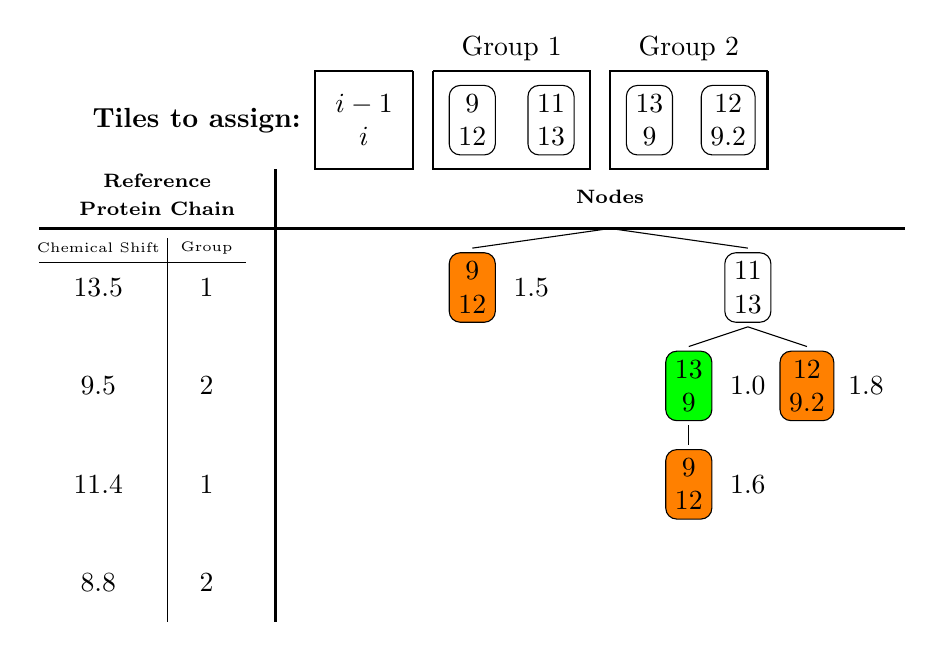
\begin{tikzpicture} [scale=.5]

		% Tile groups 
		\draw [thick] (6,6) -- (10,6) -- (10,3.5) -- (6,3.5) -- (6,6);
		\draw [thick] (14.5,6) -- (10.5,6) -- (10.5,3.5) -- (14.5,3.5) -- (14.5,6);
		\node[align=center] at (0,4.75) {\textbf{Tiles to assign:}};
		\node[align=center] at (4.25,4.75) {$i-1$\\$i$};
		\draw [thick] (5.5,6) -- (3,6) -- (3,3.5) -- (5.5,3.5) -- (5.5,6);
		\node[align=center, above] at (8,6) {Group 1};
		\node[align=center, above] at (12.5,6) {Group 2};

		% tiles
		\node[align=center, rounded corners, draw] at (7,4.75) {9\\12};
		\node[align=center, rounded corners, draw] at (9,4.75) {11\\13};
		\node[align=center, rounded corners, draw] at (11.5,4.75) {13\\9};
		\node[align=center, rounded corners, draw] at (13.5,4.75) {12\\9.2};		
		\draw [thick] (-4,2) -- (18,2);

		% title
		\node[align=right] at (10.5,2.8) {\scriptsize \textbf{Nodes}};

		%first 
		\node[align=center, rounded corners, draw, fill = orange] at (7,.5) {9\\12};
		\node[align=center] at (8.5,.5) {1.5};
		\node[align=center, rounded corners, draw] at (14,.5) {11\\13};
		%\node[align=center] at (15.5,.5) {0.5};
		\draw (10.5,2) -- (7,1.5);
		\draw (10.5,2) -- (14,1.5);

		%right side row 2
		\node[align=center, rounded corners, draw, fill = green] at (12.5,-2) {13\\9};
		\node[align=center] at (14,-2) {1.0};
		\draw (14,-.5) -- (12.5,-1);
		\node[align=center, rounded corners, draw, fill = orange] at (15.5,-2) {12\\9.2};
		\node[align=center] at (17,-2) {1.8};
		\draw (14,-.5) -- (15.5,-1);

		% right side row 3
		\draw (12.5,-3) -- (12.5,-3.5);
		\node[align=center, rounded corners, draw, fill = orange] at (12.5,-4.5) {9\\12};
		\node[align=center] at (14,-4.5) {1.6};

		% grid
		\draw [thick] (2,3.5) -- (2,-8);
		\draw  (-.75,1.75) -- (-.75,-8);
		\draw  (-4,1.125) -- (1.25,1.125);

		\node[align=right] at (-1,3.2) {\scriptsize \textbf{Reference}};
		\node[align=right] at (-1,2.5) {\scriptsize \textbf{Protein Chain}};
		\node[align=right] at (-2.5,1.5) {\tiny Chemical Shift};
		\node[align=right] at (.25,1.5) {\tiny Group};
		\node[align=right] at (-2.5,.5) {13.5};
		\node[align=right] at (-2.5,-2) {9.5};
		\node[align=right] at (-2.5,-4.5) {11.4};
		\node[align=right] at (-2.5,-7) {8.8};
		\node[align=right] at (.25,.5) {1};
		\node[align=right] at (.25,-2) {2};
		\node[align=right] at (.25,-4.5) {1};
		\node[align=right] at (.25,-7) {2};

	\end{tikzpicture}
\end{document}